% Metódy inžinierskej práce

\documentclass[10pt,twoside,slovak,a4paper]{article}

\usepackage[slovak]{babel}
%\usepackage[T1]{fontenc}
\usepackage[IL2]{fontenc} % lepšia sadzba písmena Ľ než v T1
\usepackage[utf8]{inputenc}
\usepackage{graphicx}
\usepackage{float}
\usepackage{url} % príkaz \url na formátovanie URL
\usepackage{hyperref} % odkazy v texte budú aktívne (pri niektorých triedach dokumentov spôsobuje posun textu)
\usepackage{framed}
\usepackage{cite}
%\usepackage{times}

\graphicspath{ {./img/} }

\pagestyle{headings}
\pagestyle{headings}

\title{Využitie Natural Language Processing pre lepšie učenie jazyka\thanks{Semestrálny projekt v predmete Metódy inžinierskej práce, ak. rok 2020/21, vedenie: J. Sitarčík}} 

\author{Branislav Hozza\\[2pt]
	{\small Slovenská technická univerzita v Bratislave}\\
	{\small Fakulta informatiky a informačných technológií}\\
	{\small \texttt{xhozza@stuba.sk}}
	}

\date{\small 8. október 2020} 

\begin{document}

\maketitle
%Abstrakt
\begin{abstract}
	V tejto práci sa zameriavame na zlepšenie učenia jazyka pomocou NLP \cite{litman2016natural}. 
	Výhody NLP majú bohaté využitie v učení ako napríklad prístup k obrovskému zdroju textov. 
	NLP sa dnes využíva v mnohých odvetviach či už ako nástroje na rozpoznávanie reči alebo pomocník na opravu gramatických chýb. 
	V edukačnom systéme sa dá hlavne využiť na výučbu jazykov. NLP dokáže vyhodnocovať komplexnosť textu a kontrolovať gramatiku či plagiátorstvo. 
	Tento dokument bude zameraný hlavne na možné využitia a výzvy, ktorým musíme čeliť pri využití NLP technológie. 
	Zameriam sa na to ako NLP učí o jazykoch a ako učí samotný jazyk.
\end{abstract}
%Uvod
\section{Úvod}
\begin{flushleft}
	NLP\footnote{Natural Language Processing - spracovanie prirodzeného jazyka} sa v dnešnej dobe používa takmer v každom odvetví, či už v zdravotníctve, v informatike, kontrola textu, dátová analýza, atď. 
S príchodom nových technológií ako sú napríklad Big Data, Machine learning, MOOC\footnote{Massive open online course - veľké online kurzy} sa otvorili mnoho možností, 
ako využiť NLP v praxi. V produkcii je už aktuálne mnoho aplikácii, ktoré túto technológiu využívajú pri rôznych kurzoch.
V edukačnom systéme si môžeme ukázať v zozname \ref{zoznam_1}. Táto technológia má veľký potenciál vo využití pri učení anglického jazyka 
alebo STEM\footnote{Science, technology, engineering and mathematics - veda, technológia, inžinierstov a matematika} predmetoch. 
Pri tejto forme štúdia vieme NLP využiť na kontrolu gramatiky pri písaní esejí, učenie slovíčok alebo správnej výslovnosti.
Ako najväčšiu výhodu využitia tejto technológie v praxi vidíme hodnotenie testov so skalárne veľkým počtom testovaných študentov. 
Okrem korektnosti testov sme schopní taktiež kontrolovať plagiátorstvo textu.\linebreak
Ako môžeme vidiet v obrazku Č.\ref{nlp_obrazok}, výskum v aplikovaní NLP v edukacii spočíva v opakujúcom sa cykle. 
Technologické inovácie sú inšpirované socialnymi potrebami. Technologická inovácia je najprv informovaná a následne prispieva 
do edukačnej teórie a poskytuje dáta.
\end{flushleft}


\begin{framed}
	\centering
	\begin{figure}[H]
		\begin{itemize}\label{zoznam_1}
			\item Vyučovanie linguistických predmetov.
			– napr., čítanie, písánie, rozprávanie
			\item Používanie NLP v potrebách študentov alebo učiteľov
			– napr., knihy, učebné materiály, softvér
			\item Učenie matematiky alebo fyziky
			– napr., vytváranie slovných úloch, generovanie príkladov
		\end{itemize}
		\centering Zoznam 1
	\end{figure}
\end{framed}
\begin{framed}
	\begin{figure}[H]\label{nlp_obrazok}
		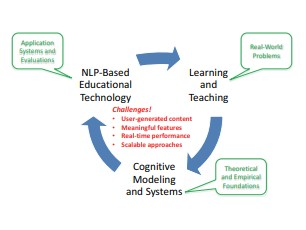
\includegraphics{nlp}
		\centering
		\caption{A picture of the universe!}
	\end{figure}
\end{framed}
%Cast o NLP
\section{Natural Language Processing} \label{NLP}
\begin{flushleft}Je to druh umelej inteligencie, zameranej na prácu s textom a obrázkami.  
Táto technológia je spojením linguistiky a informatiky, 
pričom vzniká snaha aby stroj porozumel prirodzenej reči človeka.
NLP má za sebou 70 rokov vývoja a prvé zmienky sú z roku 1950\cite{historia}.
Už v roku 1950, Alan Turing publikoval článok "Computing Machinery and Intelligence"\cite{turing2009computing} 
ktorý priniesol tzv. Turingov test ako kriterium inteligenncie, pre automatickz generovanu 
prirozdenu rec. V tej dobe sa NLP nerozlišovalo od umelej inteligencie.\linebreak
Okolo roku 2010 sa začali rozširovať metódy machine learningu ako deep learning alebo 
representation learning aj v NLP, pretože bolo dokázané že tieto techniky sú veľmi účinné.
\end{flushleft}

%Cast o uceni jazyka
\section{Učenie o jazyku} \label{ucenie_jazyka}
Jedným z najstarších a napriek tomu najaktívnejším využití NLP je jeho využitie pri učení jazyka.
Tento proces zvyčajne pozostáva vo vyhodnotení zručnosti študenta v písaní testov, v čítaní alebo
rozprávaní v danom jazyku. Syntaktická analýza sa používa na detekciu a potencialne opravenie chybného použitia
predložiek pri skupinách ako sú ESL\footnote{English as second language - ľudia pre ktorých angličtina nie je primárny jazyk.} alebo hluchý študenti.

\ldots

%Cast o uceni pomocou NLP
\section{Učenie jazyka} \label{ucenie_pomocou_nlp}
Narozdiel od využitia ako analýzy (viď. predošlá časť), jazyk môže byž využitý aj ako výučbová metóda.
V článku z roku 2011\cite{clanok_o_studovani} bolo dokázané, že skupina detí ktoré sa učia pomocou živého učiteľa, 
pochopili látku lepšie ako žiaci, ktorí sa učili pomocou PC. Hlavným rozdielom medzi ľudským učiteľom a PC učiteľom 
je, že iba človek vie používať prirodzené vety. V posledných rokoch sa systémy založené na dialógu snažia výkonovo čo najviac
priblížiť prirodzenej ľudskej reči. Uvažovalo sa aj nad tým, že učenie by sa malo odohrávať vo viac socialno 
realistickom prostredí aby sa PC učiteľ vedel viac adaptovať študentom.


\ldots

%Cast o spracovani jazyka
\section{Spracovanie jazyka} \label{spracovanie_jazyka}

\ldots


\section{Záver} \label{zaver} % prípadne iný variant názvu



\bibliography{literatura}
\bibliographystyle{plain} 
\end{document}
